% ============================================================
% CHAPTER 4 - SYSTEM ANALYSIS AND DESIGN
% ============================================================
\chapter{System Analysis and Design}
\label{ch:analysis-design}

\section{Introduction}

Chapter~\ref{ch:methodology} established how a trained phoneme error detector is
obtained. This chapter establishes what has to be built around it for that
detector to be usable by a person practising speech. It begins with stakeholder
and requirements analysis (Sections~\ref{sec:stakeholders}--\ref{sec:nfr}),
proceeds to the system architecture and its component decomposition
(Sections~\ref{sec:architecture}--\ref{sec:components}), specifies the neural
network design in detail (Section~\ref{sec:network-design}), specifies the
processing pipeline and API contract
(Sections~\ref{sec:pipeline-design}--\ref{sec:api-design}), and closes with the
user-interface design (Section~\ref{sec:ui-design}) and the design decisions
that were made and their justifications (Section~\ref{sec:design-decisions}).

\section{Stakeholder Analysis}
\label{sec:stakeholders}

\begin{description}[leftmargin=0.6cm,style=nextline]
  \item[Primary user --- a person with dysarthric or unclear speech.] Wants to
        know which sounds in a practised word came out unclear. Requires that
        the interaction be short, that the feedback be legible without technical
        knowledge, and that the tool run on a phone. May have limited fine motor
        control, which constrains the interaction to large targets and a small
        number of them.
  \item[Secondary user --- a speech-language pathologist.] Wants an objective
        signal to supplement perceptual judgement, and wants to prescribe
        between-session practice that produces feedback. Requires that the
        system's confidence be visible rather than hidden behind a binary
        verdict, and that its limitations be stated so that it is not mistaken
        for a diagnostic instrument.
  \item[Tertiary user --- a language learner or public speaker.] Wants
        per-sound feedback on articulation clarity. Is served by the same
        interface, with the caveat that the model was trained on a dysarthric
        population.
  \item[Researcher / maintainer.] Requires that the deployed feature pipeline be
        provably identical to the training pipeline, that all decision
        parameters be externally configurable, and that the system report its
        own operational state.
\end{description}

The use cases derived from these stakeholders are shown in
Figure~\ref{fig:usecase}.

\begin{figure}[H]
\centering
\begin{tikzpicture}[node distance=6mm]
  \node[actor] (user) at (0,0) {\parbox{1.2cm}{\centering Practising\\speaker}};
  \node[actor] (slp) at (0,-4.2) {\parbox{1.2cm}{\centering SLP}};

  \begin{scope}[every node/.style={ellipse, draw=black!70, fill=blue!5,
                 minimum width=4.4cm, minimum height=0.95cm, font=\scriptsize,
                 align=center}]
    \node (uc1) at (5.2, 1.2)  {Select / enter a target word};
    \node (uc2) at (5.2, 0.0)  {Record the word from the microphone};
    \node (uc3) at (5.2,-1.2)  {Upload an existing audio file};
    \node (uc4) at (5.2,-2.4)  {View the per-phoneme verdicts};
    \node (uc5) at (5.2,-3.6)  {View the clarity score and waveform};
    \node (uc6) at (5.2,-4.8)  {Adjust the sensitivity threshold};
    \node (uc7) at (5.2,-6.0)  {Check service health status};
  \end{scope}

  \node[draw=black!55, dashed, rounded corners, fit=(uc1)(uc7),
        inner sep=8pt, label={[font=\small]above:\textbf{\systemName}}] {};

  \foreach \t in {uc1,uc2,uc3,uc4,uc5,uc6} \draw[thick, black!60] (user) -- (\t);
  \foreach \t in {uc4,uc5,uc6,uc7} \draw[thick, black!60] (slp) -- (\t);
\end{tikzpicture}
\caption[Use case diagram]{Use case diagram for the \systemName\ system.}
\label{fig:usecase}
\end{figure}

\section{Functional Requirements}
\label{sec:fr}

\begin{table}[H]
\centering
\caption[Functional requirements]{Functional requirements.}
\label{tab:fr}
\small
\begin{tabularx}{\textwidth}{@{}p{1.1cm}Xp{1.5cm}@{}}
\toprule
\textbf{ID} & \textbf{Requirement} & \textbf{Priority} \\
\midrule
FR-01 & The system shall accept a target word or short phrase as free text. & Must \\
FR-02 & The system shall offer a set of suggested practice words. & Should \\
FR-03 & The system shall record audio from the device microphone in the browser. & Must \\
FR-04 & The system shall accept an uploaded audio file as an alternative to recording. & Must \\
FR-05 & The system shall resample captured audio to 16\,kHz mono before submission. & Must \\
FR-06 & The system shall derive the canonical IPA phoneme sequence for the target word. & Must \\
FR-07 & The system shall force-align the recording to that phoneme sequence and return time boundaries. & Must \\
FR-08 & The system shall classify each aligned phoneme as \emph{correct} or \emph{error}. & Must \\
FR-09 & The system shall return a continuous error probability for each phoneme alongside the binary verdict. & Must \\
FR-10 & The system shall return an overall clarity score for the utterance. & Must \\
FR-11 & The system shall return a downsampled waveform for client-side visualisation. & Should \\
FR-12 & The system shall render the waveform with each phoneme span shaded by its verdict. & Should \\
FR-13 & The system shall allow the user to adjust the error-probability threshold within a bounded range. & Should \\
FR-14 & The system shall reject recordings that are silent, too quiet or noise-dominated, with an actionable message. & Must \\
FR-15 & The system shall detect when a word other than the target was spoken and report this distinctly from a mispronunciation. & Should \\
FR-16 & The system shall expose a health endpoint reporting model, aligner and G2P availability. & Must \\
FR-17 & The system shall allow playback of the submitted recording. & Could \\
FR-18 & The system shall support a light and a dark visual theme. & Could \\
\bottomrule
\end{tabularx}
\end{table}

\section{Non-Functional Requirements}
\label{sec:nfr}

\begin{table}[H]
\centering
\caption[Non-functional requirements]{Non-functional requirements.}
\label{tab:nfr}
\small
\begin{tabularx}{\textwidth}{@{}p{1.2cm}p{2.5cm}X@{}}
\toprule
\textbf{ID} & \textbf{Category} & \textbf{Requirement} \\
\midrule
NFR-01 & Performance & A single-word analysis shall complete within 5\,s on a 2-vCPU host once models are warm. \\
NFR-02 & Performance & Models shall be loaded once at process start and reused, never per request. \\
NFR-03 & Correctness & The inference feature pipeline shall be numerically identical to the training pipeline, including the global normalisation constants. \\
NFR-04 & Portability & The system shall run on CPU-only hardware with no GPU requirement. \\
NFR-05 & Portability & The system shall deploy as a single container image on a free-tier host. \\
NFR-06 & Usability & The primary interaction shall be reachable in at most two taps from the landing view. \\
NFR-07 & Usability & The interface shall be usable on a mobile viewport of 360\,px width. \\
NFR-08 & Accessibility & Verdicts shall not be conveyed by colour alone. \\
NFR-09 & Reliability & Failure of an optional component shall degrade the service rather than disable it. \\
NFR-10 & Security & Uploads shall be size-limited and CORS origins shall be configurable. \\
NFR-11 & Privacy & Audio shall be processed in memory and never persisted to disk. \\
NFR-12 & Maintainability & All decision parameters shall be settable by environment variable without a rebuild. \\
NFR-13 & Observability & The service shall report its own readiness and degradation state. \\
\bottomrule
\end{tabularx}
\end{table}

\section{System Architecture}
\label{sec:architecture}

The trained classifier that Chapter~\ref{ch:methodology} produces
(Figure~\ref{fig:method-pipeline}) is deployed inside a three-tier
architecture: a presentation tier in the browser, an application tier hosting
the inference service, and a model tier holding the trained artefacts and the
pre-trained acoustic models (Figure~\ref{fig:architecture}).

The decisive constraint on this decomposition is that the classifier is a
TensorFlow model, the aligner is a PyTorch model and the G2P engine is a native
binary. None of these can run in a browser, so all inference is server-side and
the client's responsibilities are confined to capture, format conversion,
submission and presentation. The corresponding cost --- a network round trip
carrying the audio payload --- is acceptable because a single-word recording
is only tens of kilobytes at 16\,kHz mono.

\begin{figure}[H]
\centering
\begin{tikzpicture}[node distance=6mm and 9mm]

% ---- presentation tier ----
\node[block] (rec)  {Recorder \\ \scriptsize MediaRecorder API};
\node[block, right=of rec] (conv) {WAV encoder \\ \scriptsize 16\,kHz mono PCM16};
\node[block, right=of conv] (view) {Result views \\ \scriptsize waveform, ring, list};
\node[draw=black!55, rounded corners, dashed, fit=(rec)(conv)(view), inner sep=7pt] (tier1) {};
\node[font=\small\bfseries, anchor=west] at ([xshift=2pt,yshift=-2pt]tier1.north west) {Presentation tier — React PWA};

% ---- application tier ----
\node[block, below=20mm of rec] (api) {FastAPI router \\ \scriptsize /api/analyze, /api/health};
\node[block, right=of api] (gate) {Quality gate \\ \scriptsize RMS, spectral flatness};
\node[block, right=of gate] (verify) {Word verifier \\ \scriptsize Whisper + similarity};
\node[wideblock, below=8mm of gate] (pipe) {Inference pipeline \\ \scriptsize trim $\rightarrow$ G2P $\rightarrow$ align $\rightarrow$ mel $\rightarrow$ classify};
\node[draw=black!55, rounded corners, dashed, fit=(api)(gate)(verify)(pipe), inner sep=7pt] (tier2) {};
\node[font=\small\bfseries, anchor=west] at ([xshift=2pt,yshift=-2pt]tier2.north west) {Application tier — FastAPI service};

% ---- model tier ----
\node[data, below=18mm of pipe] (w2v) {wav2vec2 aligner \\ \scriptsize frozen CTC phone model};
\node[data, left=of w2v] (keras) {CNN--BiLSTM \\ \scriptsize .keras, 415{,}810 params};
\node[data, right=of w2v] (whis) {Whisper tiny.en \\ \scriptsize word verification};
\node[data, below=7mm of w2v] (esp) {espeak-ng binary + mel normalisation constants};
\node[draw=black!55, rounded corners, dashed, fit=(keras)(w2v)(whis)(esp), inner sep=7pt] (tier3) {};
\node[font=\small\bfseries, anchor=west] at ([xshift=2pt,yshift=-2pt]tier3.north west) {Model tier — artefacts};

\draw[arrow] (tier1.south) -- node[lbl] {\scriptsize HTTPS multipart: WAV + word} (tier2.north);
\draw[arrow] (tier2.south) -- node[lbl] {\scriptsize in-process calls} (tier3.north);
\draw[dashedarrow] (tier2.west) -- ++(-1.0,0) |- node[lbl, near start] {\scriptsize JSON verdicts} (tier1.west);
\end{tikzpicture}
\caption[System architecture]{Three-tier architecture of the \systemName\
system.}
\label{fig:architecture}
\end{figure}

\section{Component Design}
\label{sec:components}

\subsection{Presentation tier}

\begin{description}[leftmargin=0.6cm,style=nextline]
  \item[\texttt{App}] Root component holding the application state: target word,
        interaction status, threshold, result and service health.
  \item[\texttt{Recorder} / \texttt{toWav16k}] Audio capture and format
        conversion. The browser's \texttt{MediaRecorder} emits WebM/Opus, which
        the server-side decoder cannot read without \texttt{ffmpeg}. The client
        therefore decodes the recording with the Web Audio API, resamples to
        16\,kHz mono through an \texttt{OfflineAudioContext} and hand-encodes a
        16-bit PCM WAV. Placing this conversion on the client removes a heavy
        native dependency from the server and guarantees that the server always
        receives the exact format the training pipeline assumed.
  \item[\texttt{WaveformChart}] Draws the returned waveform and shades each
        phoneme's time span according to its verdict.
  \item[\texttt{PhonemeList}] Tabulates each phoneme with its verdict and an
        error-probability meter.
  \item[\texttt{ScoreRing}] Renders the overall clarity score as a radial
        progress indicator.
  \item[\texttt{ThresholdSlider}] Exposes the decision threshold within the
        bounds permitted by the server.
  \item[\texttt{ThemeToggle}] Light/dark theme selection persisted locally.
\end{description}

\subsection{Application tier}

\begin{description}[leftmargin=0.6cm,style=nextline]
  \item[\texttt{main}] HTTP routing, request validation, error mapping and the
        start-up warm-up hook that loads all models before the first request.
  \item[\texttt{audio}] Decoding of arbitrary uploaded bytes to a mono float
        waveform, silence trimming, the quality assessment described below, and
        peak-preserving downsampling of the waveform for client display.
  \item[\texttt{phonemes}] G2P via the \texttt{espeak-ng} subprocess, with
        diacritic stripping identical to training.
  \item[\texttt{pipeline}] The inference pipeline proper, holding the lazily
        loaded models behind a lock and exposing \texttt{align},
        \texttt{crop\_mel}, \texttt{verify\_word} and \texttt{analyze}.
  \item[\texttt{config}] A single typed settings object, populated from
        environment variables, holding every parameter of
        Table~\ref{tab:feature-params} together with the decision thresholds.
  \item[\texttt{schemas}] Response models, which also generate the API
        documentation.
\end{description}

\section{Neural Network Design}
\label{sec:network-design}

\subsection{Rationale}

The input is a $64 \times 32 \times 1$ log-mel patch. Two design decisions
follow from its structure.

Convolution is applied first because the discriminative content of the patch is
\emph{local} in time--frequency: a weak stop release, a missing fricative noise
band or a smeared formant transition are localised spectro-temporal events, and
their significance does not depend on where in the patch they occur. Two
convolutional blocks with $3\times3$ kernels give a receptive field sufficient
to span a formant transition after pooling, while keeping the parameter count
small.

A recurrent stage follows because a phoneme's quality is carried by its
\emph{trajectory}. After the convolutional blocks the tensor is
$16 \times 8 \times 32$; a \texttt{TimeDistributed} flatten reinterprets this as
a sequence of 16 time steps each carrying a 256-dimensional feature vector, and
the bidirectional LSTM integrates that sequence. Bidirectionality is appropriate
because the entire phoneme segment is available at inference time --- this is
not a streaming task --- and because the interpretation of a release depends on
the closure that preceded it and vice versa.

\subsection{Layer specification}

The selected architecture is specified in Table~\ref{tab:model-layers} and drawn
in Figure~\ref{fig:network}.

\begin{table}[H]
\centering
\caption[CNN--BiLSTM layer specification]{Layer-by-layer specification of the
selected CNN--BiLSTM classifier.}
\label{tab:model-layers}
\small
\begin{tabular}{@{}llrp{4.6cm}@{}}
\toprule
\textbf{Layer} & \textbf{Output shape} & \textbf{Params} & \textbf{Configuration} \\
\midrule
Input                    & $64\times32\times1$   & 0        & log-mel patch \\
Conv2D                   & $64\times32\times16$  & 160      & $3\times3$, ReLU, \texttt{same} \\
BatchNormalization       & $64\times32\times16$  & 64       & \\
MaxPooling2D             & $32\times16\times16$  & 0        & $2\times2$ \\
Dropout                  & $32\times16\times16$  & 0        & $p=0.3$ \\
Conv2D                   & $32\times16\times32$  & 4{,}640  & $3\times3$, ReLU, \texttt{same} \\
BatchNormalization       & $32\times16\times32$  & 128      & \\
MaxPooling2D             & $16\times8\times32$   & 0        & $2\times2$ \\
Dropout                  & $16\times8\times32$   & 0        & $p=0.3$ \\
TimeDistributed(Flatten) & $16\times256$         & 0        & sequence of 16 steps \\
Bidirectional(LSTM)      & $256$                 & 394{,}240& 128 units per direction, $p=0.3$ \\
Dense                    & $64$                  & 16{,}448 & ReLU \\
Dropout                  & $64$                  & 0        & $p=0.3$ \\
Dense                    & $2$                   & 130      & softmax \\
\midrule
\multicolumn{2}{@{}l}{\textbf{Total parameters}}  & \textbf{415{,}810} & (1.59\,MB) \\
\multicolumn{2}{@{}l}{Trainable}                  & 415{,}714 & \\
\multicolumn{2}{@{}l}{Non-trainable}              & 96        & batch-norm statistics \\
\bottomrule
\end{tabular}
\end{table}

\begin{figure}[H]
\centering
\begin{tikzpicture}[node distance=4.5mm, every node/.style={font=\scriptsize}]
  \tikzset{
    lyr/.style={rectangle, rounded corners=2pt, draw=black!70, minimum height=0.72cm,
                text width=3.5cm, align=center, inner sep=3pt},
    inl/.style={lyr, fill=green!10},
    cnl/.style={lyr, fill=blue!10},
    rnl/.style={lyr, fill=orange!14},
    dnl/.style={lyr, fill=purple!10},
    outl/.style={lyr, fill=red!10},
    dim/.style={font=\scriptsize\itshape, anchor=west, text=black!60},
  }
  \node[inl] (i)  {Input log-mel patch};
  \node[cnl, below=of i]  (c1) {Conv2D 16 @ $3{\times}3$ + BN + MaxPool + Dropout};
  \node[cnl, below=of c1] (c2) {Conv2D 32 @ $3{\times}3$ + BN + MaxPool + Dropout};
  \node[rnl, below=of c2] (td) {TimeDistributed(Flatten)};
  \node[rnl, below=of td] (bi) {Bidirectional LSTM (128 units/dir)};
  \node[dnl, below=of bi] (d1) {Dense 64, ReLU + Dropout};
  \node[outl, below=of d1] (d2) {Dense 2, softmax};
  \node[below=of d2, font=\scriptsize] (out) {$P(\text{correct}),\ P(\text{error})$};

  \foreach \a/\b in {i/c1, c1/c2, c2/td, td/bi, bi/d1, d1/d2, d2/out}
    \draw[arrow] (\a) -- (\b);

  \node[dim] at ([xshift=4mm]i.east)  {$64\times32\times1$};
  \node[dim] at ([xshift=4mm]c1.east) {$32\times16\times16$};
  \node[dim] at ([xshift=4mm]c2.east) {$16\times8\times32$};
  \node[dim] at ([xshift=4mm]td.east) {$16\times256$};
  \node[dim] at ([xshift=4mm]bi.east) {$256$};
  \node[dim] at ([xshift=4mm]d1.east) {$64$};
  \node[dim] at ([xshift=4mm]d2.east) {$2$};
\end{tikzpicture}
\caption[CNN--BiLSTM architecture]{The selected CNN--BiLSTM classifier. Tensor
shapes are annotated to the right of each stage.}
\label{fig:network}
\end{figure}

\section{Processing Pipeline Design}
\label{sec:pipeline-design}

Figure~\ref{fig:sequence} traces a single analysis request through the system.
Two stages exist in the deployed pipeline that have no counterpart in the
training notebook, and both were added because a deployed system receives
inputs that a curated corpus does not.

\textbf{The quality gate} rejects a recording before any model is invoked if it
is empty, if its RMS level is below $-40$\,dBFS (silence or a microphone that
was not actually capturing), or if its mean spectral flatness exceeds $0.6$
(broadband noise rather than speech). Without this gate the pipeline would
happily align phonemes to room tone and return a confident set of verdicts
about nothing, which is both misleading and a waste of compute.

\textbf{Target-word verification} distinguishes two situations that produce very
similar model output but require opposite feedback. If the user says an entirely
different word, the forced aligner --- being constrained --- will still place
the target phonemes somewhere in the audio, and the classifier will report a
large number of errors. The correct response is ``you said a different word'',
not ``your pronunciation was poor''. A small Whisper model transcribes the
recording, both transcript and target are passed through Whisper's text
normaliser, and the maximum similarity ratio between the target and any
transcribed word is compared against a threshold. This is deliberately a
\emph{coarse} check: it is not a pronunciation judge, only a guard against the
wrong-word case, and its threshold is set permissively so that a heavily
distorted but genuine attempt is not rejected.

\begin{figure}[H]
\centering
\resizebox{\textwidth}{!}{%
\begin{tikzpicture}[font=\scriptsize]
  \def\lx{0} \def\ax{3.6} \def\gx{6.6} \def\wx{9.4} \def\px{12.2}
  \def\ytop{0} \def\ybot{-11.4}

  \foreach \x/\n in {\lx/{Browser}, \ax/{API}, \gx/{Quality gate}, \wx/{Whisper}, \px/{Pipeline}} {
    \node[draw=black!70, fill=blue!6, rounded corners=2pt, minimum width=1.9cm,
          minimum height=0.6cm, align=center] at (\x,\ytop) {\n};
    \draw[dashed, black!45] (\x,\ytop-0.35) -- (\x,\ybot);
  }

  \newcommand{\msg}[4]{\draw[arrow] (#1,#3) -- node[above, font=\tiny, fill=white, inner sep=1pt] {#4} (#2,#3);}
  \newcommand{\rmsg}[4]{\draw[dashedarrow] (#1,#3) -- node[above, font=\tiny, fill=white, inner sep=1pt] {#4} (#2,#3);}

  \msg{\lx}{\ax}{-1.1}{POST /api/analyze (WAV + word)}
  \node[right, font=\tiny, text=black!60] at (\ax+0.15,-1.75) {validate word, size, threshold bounds};
  \msg{\ax}{\gx}{-2.4}{decode, resample, trim}
  \rmsg{\gx}{\ax}{-3.1}{ok \textbar\ 422 too quiet / noise}
  \msg{\ax}{\wx}{-3.9}{verify target word}
  \rmsg{\wx}{\ax}{-4.6}{heard + similarity}
  \node[right, font=\tiny, text=black!60] at (\ax+0.15,-5.25) {if mismatch $\rightarrow$ 422 ``you said \dots''};
  \msg{\ax}{\px}{-5.9}{analyze(wave, word, threshold)}
  \node[right, font=\tiny, text=black!60, align=left] at (\px-3.3,-6.6)
       {espeak-ng G2P $\rightarrow$ wav2vec2 emission $\rightarrow$ forced align};
  \node[right, font=\tiny, text=black!60, align=left] at (\px-3.3,-7.2)
       {crop + mel + global $z$-score $\rightarrow$ batched CNN--BiLSTM predict};
  \rmsg{\px}{\ax}{-8.0}{per-phoneme $P(\text{error})$}
  \node[right, font=\tiny, text=black!60] at (\ax+0.15,-8.65) {apply threshold, compute clarity score, downsample waveform};
  \rmsg{\ax}{\lx}{-9.6}{200 JSON: phonemes, score, waveform}
  \node[right, font=\tiny, text=black!60] at (\lx+0.15,-10.3) {render ring, shaded waveform, phoneme list};
\end{tikzpicture}}
\caption[Analysis request sequence]{Sequence of a single \texttt{/api/analyze}
request. The quality gate and the word verifier are deployment-only stages with
no counterpart in the training notebook.}
\label{fig:sequence}
\end{figure}

\section{API Design}
\label{sec:api-design}

The service exposes the two endpoints of Table~\ref{tab:api}. The response
schema is designed so that the client needs no knowledge of the model: it
receives absolute times in the same timebase as the returned waveform, and both
a binary verdict and a continuous probability for every phoneme.

\begin{table}[H]
\centering
\caption[API endpoints]{API endpoints.}
\label{tab:api}
\small
\begin{tabularx}{\textwidth}{@{}p{1.5cm}p{2.4cm}p{3.3cm}X@{}}
\toprule
\textbf{Method} & \textbf{Path} & \textbf{Request} & \textbf{Response} \\
\midrule
GET  & \texttt{/api/health}  & --- & \texttt{status}, \texttt{model\_loaded}, \texttt{align\_model\_loaded}, \texttt{whisper\_loaded}, \texttt{espeak\_available}, \texttt{device}, \texttt{normalization} \\
POST & \texttt{/api/analyze} & multipart: \texttt{audio} (file), \texttt{target\_word} (text), \texttt{error\_threshold} (optional float) & \texttt{target\_word}, \texttt{phonemes[]}, \texttt{n\_errors}, \texttt{n\_phonemes}, \texttt{accuracy}, \texttt{duration\_sec}, \texttt{error\_threshold}, \texttt{waveform[]}, \texttt{waveform\_rate} \\
\bottomrule
\end{tabularx}
\end{table}

Each element of \texttt{phonemes[]} carries \texttt{phoneme} (IPA symbol),
\texttt{start} and \texttt{end} (seconds, trimmed timebase), \texttt{verdict}
(\texttt{"ERROR"} or \texttt{"ok"}), \texttt{error\_prob} and
\texttt{align\_score}. The alignment confidence is surfaced deliberately: a
phoneme with a very low alignment score should be interpreted cautiously,
because it may indicate that the sound was omitted entirely rather than
mispronounced.

Error responses follow a consistent discipline. HTTP 422 signals a problem with
the \emph{input} that the user can fix (empty word, undecodable audio, audio too
quiet, noise rather than speech, wrong word spoken, no phonemes alignable), and
the detail string is written as user-facing guidance. HTTP 503 signals a
degraded \emph{service} (G2P binary missing, model unavailable). HTTP 413 signals
an oversized upload. HTTP 500 is reserved for genuinely unexpected failures.

\section{User Interface Design}
\label{sec:ui-design}

The interface is a single scrolling view organised into a prompt card and a
result card (Figure~\ref{fig:ui}). The design targets NFR-06 and NFR-07: the
primary action is reachable in one tap from the landing state, and the layout
reflows to a single column on narrow viewports.

Four decisions govern the presentation of results.

\textbf{The clarity score is shown first and largest}, as a radial ring, because
a single legible number is what tells the user whether the attempt was better
than the last one.

\textbf{Verdicts are anchored in time on the waveform.} Shading each phoneme's
interval directly on the signal connects the abstract verdict to the moment in
the recording at which it applies, which is what makes the feedback actionable
during repeated practice.

\textbf{Uncertainty is exposed rather than hidden.} Each phoneme's row carries a
probability meter as well as a verdict, so a marginal case at $P = 0.51$ is
visually distinguishable from a confident one at $P = 0.95$. Presenting only the
binary verdict would overstate the model's certainty --- which, given the
proxy-label limitation of Section~\ref{sec:limitations}, would be misleading.

\textbf{Colour is never the sole carrier of meaning} (NFR-08): every verdict is
also expressed as text and as a meter position.

\begin{figure}[H]
\centering
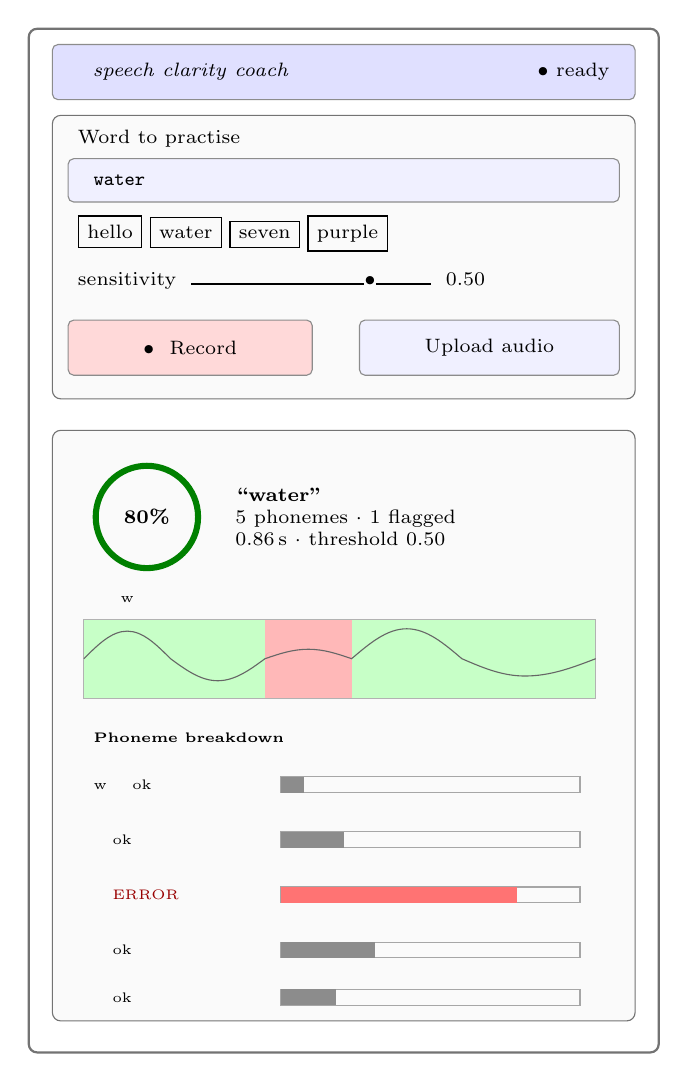
\begin{tikzpicture}[font=\scriptsize, x=1cm, y=1cm]
  \tikzset{
    panel/.style={draw=black!55, rounded corners=3pt, fill=gray!4},
    ctl/.style={draw=black!45, rounded corners=2pt, fill=blue!6},
  }
  % ---- device frame ----
  \draw[panel, fill=white, thick] (0,0) rectangle (8,13);

  % ---- header ----
  \draw[ctl, fill=blue!12] (0.3,12.1) rectangle (7.7,12.8);
  \node[anchor=west] at (0.5,12.45) {\textbf{\systemName} \ \emph{speech clarity coach}};
  \node[anchor=east] at (7.5,12.45) {$\bullet$ ready};

  % ---- prompt card ----
  \draw[panel] (0.3,8.3) rectangle (7.7,11.9);
  \node[anchor=west] at (0.5,11.6) {Word to practise};
  \draw[ctl] (0.5,10.8) rectangle (7.5,11.35);
  \node[anchor=west] at (0.7,11.08) {\texttt{water}};
  \node[anchor=west] at (0.5,10.4) {\fbox{hello} \fbox{water} \fbox{seven} \fbox{purple}};
  \node[anchor=west] at (0.5,9.8)
       {sensitivity \ \rule{2.2cm}{1pt}$\bullet$\rule{0.7cm}{1pt} \ 0.50};
  \draw[ctl, fill=red!15] (0.5,8.6) rectangle (3.6,9.3);
  \node at (2.05,8.95) {$\bullet$ \ Record};
  \draw[ctl] (4.2,8.6) rectangle (7.5,9.3);
  \node at (5.85,8.95) {Upload audio};

  % ---- result card ----
  \draw[panel] (0.3,0.4) rectangle (7.7,7.9);
  \draw[line width=2.2pt, green!50!black] (1.5,6.8) circle (0.65);
  \node[font=\scriptsize\bfseries] at (1.5,6.8) {80\%};
  \node[anchor=west, align=left] at (2.5,6.8)
       {\textbf{``water''}\\ 5 phonemes $\cdot$ 1 flagged\\ 0.86\,s $\cdot$ threshold 0.50};

  % ---- waveform with verdict shading ----
  \fill[green!22] (0.7,4.5) rectangle (1.8,5.5);
  \fill[green!22] (1.8,4.5) rectangle (3.0,5.5);
  \fill[red!28]   (3.0,4.5) rectangle (4.1,5.5);
  \fill[green!22] (4.1,4.5) rectangle (5.5,5.5);
  \fill[green!22] (5.5,4.5) rectangle (7.2,5.5);
  \draw[black!30] (0.7,4.5) rectangle (7.2,5.5);
  \draw[black!60] (0.7,5.0) sin (1.25,5.35) cos (1.8,5.0) sin (2.4,4.72)
                  cos (3.0,5.0) sin (3.55,5.12) cos (4.1,5.0) sin (4.8,5.38)
                  cos (5.5,5.0) sin (6.3,4.78) cos (7.2,5.0);
  \node[font=\tiny] at (1.25,5.75) {w};
  \node[font=\tiny] at (2.40,5.75) {\textscripta};
  \node[font=\tiny, text=red!60!black] at (3.55,5.75) {\textfishhookr};
  \node[font=\tiny] at (4.80,5.75) {\textrhookschwa};
  \node[font=\tiny] at (6.35,5.75) {\textturnr};

  % ---- phoneme breakdown ----
  \node[anchor=west, font=\tiny\bfseries] at (0.7,4.0) {Phoneme breakdown};
  % row 1
  \node[anchor=west, font=\tiny] at (0.7,3.4) {w \quad ok};
  \draw[black!35] (3.2,3.3) rectangle (7.0,3.5);
  \fill[black!45] (3.2,3.3) rectangle (3.5,3.5);
  % row 2
  \node[anchor=west, font=\tiny] at (0.7,2.7) {\textscripta \quad ok};
  \draw[black!35] (3.2,2.6) rectangle (7.0,2.8);
  \fill[black!45] (3.2,2.6) rectangle (4.0,2.8);
  % row 3
  \node[anchor=west, font=\tiny, text=red!60!black] at (0.7,2.0) {\textfishhookr \quad ERROR};
  \draw[black!35] (3.2,1.9) rectangle (7.0,2.1);
  \fill[red!55]   (3.2,1.9) rectangle (6.2,2.1);
  % row 4
  \node[anchor=west, font=\tiny] at (0.7,1.3) {\textrhookschwa \quad ok};
  \draw[black!35] (3.2,1.2) rectangle (7.0,1.4);
  \fill[black!45] (3.2,1.2) rectangle (4.4,1.4);
  % row 5
  \node[anchor=west, font=\tiny] at (0.7,0.7) {\textturnr \quad ok};
  \draw[black!35] (3.2,0.6) rectangle (7.0,0.8);
  \fill[black!45] (3.2,0.6) rectangle (3.9,0.8);
\end{tikzpicture}
\caption[User interface design]{Interface layout on a mobile viewport: prompt
card above, result card below, with the clarity ring, the verdict-shaded
waveform and the per-phoneme breakdown with probability meters.}
\label{fig:ui}
\end{figure}

\section{Key Design Decisions and Justifications}
\label{sec:design-decisions}

\subsection{Server-side inference}

\emph{Decision.} All model execution occurs on the server; the client performs
capture, conversion and rendering only.

\emph{Justification.} The three model components are a TensorFlow graph, a
PyTorch transformer and a native binary; none has a viable in-browser
equivalent that would preserve numerical equivalence with training. Porting the
classifier alone to a browser runtime would not help, because the aligner and
the G2P engine would still be server-side. The cost is a round trip carrying
tens of kilobytes, which is negligible relative to the inference time itself.

\subsection{Client-side format conversion}

\emph{Decision.} The browser converts recorded audio to 16\,kHz mono PCM16 WAV
before upload.

\emph{Justification.} Browsers record WebM/Opus, which \texttt{libsndfile}
cannot decode; the server-side fallback path requires \texttt{ffmpeg}, a large
native dependency. Converting on the client removes that dependency, reduces
the upload size, and guarantees the server receives exactly the format the
training pipeline assumed.

\subsection{A user-adjustable decision threshold}
\label{sec:design-threshold}

\emph{Decision.} The error-probability threshold defaults to $0.50$ and is
adjustable by the user within $[0.30, 0.70]$, with the bounds enforced
server-side.

\emph{Justification.} The appropriate operating point is not a property of the
model but of the use case. A clinician screening for targets wants sensitivity
and will lower the threshold; a user practising a sound they have nearly
mastered wants precision and will raise it. Exposing the threshold also serves
an honesty function --- it makes visible that the verdict is a tunable decision
rather than an objective fact. The bounds are enforced server-side so that the
control cannot be pushed into a degenerate regime where everything or nothing
is flagged.

\subsection{Baked-in normalisation constants}

\emph{Decision.} The global mel mean and standard deviation are resolved with a
three-level precedence: environment variables, then the dataset archive if
present, then constants compiled into the configuration module.

\emph{Justification.} These two scalars are part of the trained model
(Section~\ref{sec:features}). Shipping the 54\,MB dataset archive purely to
recover two floating-point numbers is wasteful, and making the service silently
fall back to per-clip normalisation when the archive is absent would produce a
service that runs but is quietly less accurate --- the worst possible failure
mode. Compiling the values in makes the correct behaviour the default, while
the environment-variable override preserves the ability to retrain.

\subsection{Graceful degradation}

\emph{Decision.} Optional components degrade the service rather than disabling
it, and the health endpoint reports the degraded state.

\emph{Justification.} Whisper-based verification is a convenience; if it fails
to load or throws, analysis proceeds without it. Model warm-up failure at start
--- typically a transient network problem while fetching the aligner --- is
logged and retried on first request rather than crashing the process. The
health endpoint distinguishes \emph{ready}, \emph{degraded} and \emph{offline},
and the client surfaces that state so a user is never left interpreting an
unexplained failure.
